% Closed-loop validation as implemented (meeting-07-09-2026/code/common.py docstring,
% closed_loop.py): u = u_data + C_fb(y_data - y_model); the model state is never reset to data.
\documentclass[border=8pt]{standalone}
% Shared preamble of the TikZ slide figures. Role colours match style.py.
\usepackage[T1]{fontenc}
\usepackage[scaled]{helvet}
\renewcommand\familydefault{\sfdefault}
\usepackage{amsmath}
\usepackage{tikz}
\usetikzlibrary{arrows.meta,calc,decorations.pathmorphing,positioning}
\definecolor{cbase}{HTML}{D55E00}   % physics model
\definecolor{caug}{HTML}{0072B2}    % augmented model, no projection
\definecolor{cproj}{HTML}{009E73}   % augmented model with projection
\definecolor{cink}{HTML}{222222}
\definecolor{cmuted}{HTML}{6B6B6B}

\begin{document}
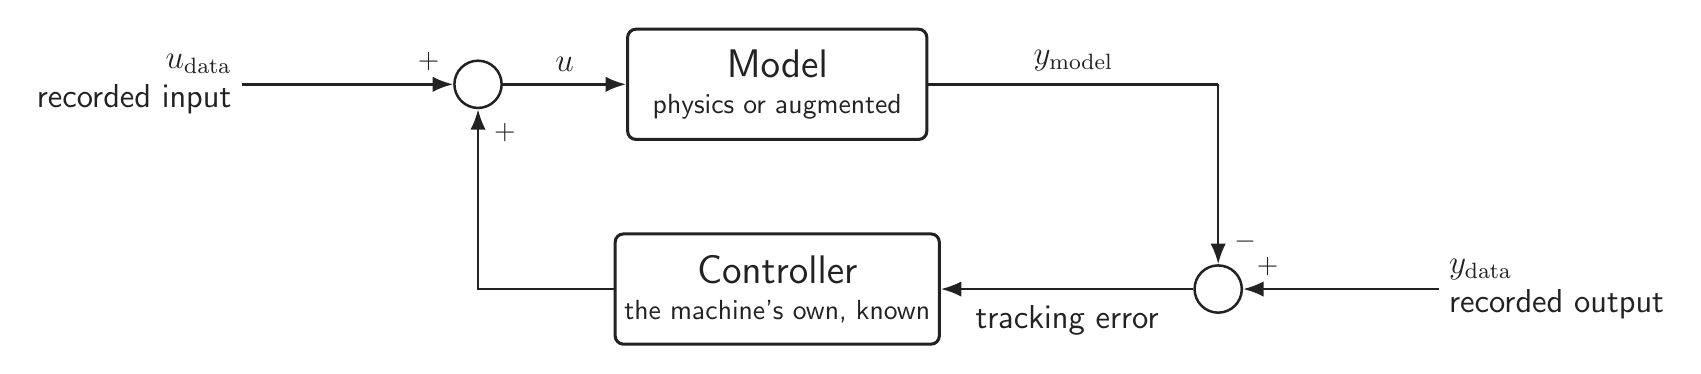
\begin{tikzpicture}[
    >={Latex[length=2.6mm]},
    sig/.style={->, line width=0.9pt, draw=cink},
    blk/.style={draw=cink, line width=1.1pt, rounded corners=3pt, align=center,
                minimum height=14mm, minimum width=38mm, text=cink, fill=white},
    sum/.style={draw=cink, line width=0.9pt, circle, inner sep=0pt, minimum size=6mm},
    lbl/.style={font=\large, text=cink},
    sgn/.style={font=\normalsize, text=cink},
  ]
  \node[sum] (S1) at (0,0) {};
  \node[blk] (M) at (3.8,0) {\Large Model\\[1pt]\normalsize physics or augmented};
  \coordinate (T) at (9.4,0);
  \node[sum] (S2) at (9.4,-2.6) {};
  \node[blk] (C) at (3.8,-2.6) {\Large Controller\\[1pt]\normalsize the machine's own, known};

  \draw[sig] (-3.0,0) node[lbl, anchor=east, align=right] {$u_\mathrm{data}$\\recorded input}
             -- (S1.west);
  \draw[sig] (S1.east) -- node[lbl, above=1pt] {$u$} (M.west);
  \draw[line width=0.9pt, draw=cink] (M.east) -- node[lbl, above=1pt] {$y_\mathrm{model}$} (T);
  \draw[sig] (T) -- (S2.north);
  \draw[sig] (12.2,-2.6) node[lbl, anchor=west, align=left] {$y_\mathrm{data}$\\recorded output}
             -- (S2.east);
  \draw[sig] (S2.west) -- node[lbl, below=2pt] {tracking error} (C.east);
  \draw[sig] (C.west) -| (S1.south);

  \node[sgn, anchor=south east] at ($(S1.west)+(-0.05,0.05)$) {$+$};
  \node[sgn, anchor=north west] at ($(S1.south)+(0.08,-0.05)$) {$+$};
  \node[sgn, anchor=south west] at ($(S2.east)+(0.05,0.05)$) {$+$};
  \node[sgn, anchor=south west] at ($(S2.north)+(0.08,0.05)$) {$-$};
\end{tikzpicture}
\end{document}
